\chapter{Satzspiegeltest}
\label{chap:satzspiegeltest}

Weit hinten, hinter den Wortbergen, fern der L?nder Vokalien und Konsonantien leben die Blindtexte. Abgeschieden wohnen Sie in Buchstabhausen an der K?ste des Semantik, eines gro?en Sprachozeans. Ein kleines B?chlein namens Duden flie?t durch ihren Ort und versorgt sie mit den n?tigen Regelialien. Es ist ein paradiesmatisches Land, in dem einem gebratene Satzteile in den Mund fliegen. Nicht einmal von der allm?chtigen Interpunktion werden die Blindtexte beherrscht ? ein geradezu unorthographisches Leben. Eines Tages aber beschlo? eine kleine Zeile Blindtext, ihr Name war Lorem Ipsum, hinaus zu gehen in die weite Grammatik.

\section{Der gro?e Oxmox}
\label{sec:satzspiegeltest_ombox}

Der gro?e Oxmox riet ihr davon ab, da es dort wimmele von b?sen Kommata, wilden Fragezeichen und hinterh?ltigen Semikoli, doch das Blindtextchen lie? sich nicht beirren. Es packte seine sieben Versalien, schob sich sein Initial in den G?rtel und machte sich auf den Weg. Als es die ersten H?gel des Kursivgebirges erklommen hatte, warf es einen letzten Blick zur?ck auf die Skyline seiner Heimatstadt Buchstabhausen, die Headline von Alphabetdorf und die Subline seiner eigenen Stra?e, der Zeilengasse. Wehm?tig lief ihm eine rethorische Frage ?ber die Wange, dann setzte es seinen Weg fort. Unterwegs traf es eine Copy.

\begin{equation}
	\mathcal{N}(x \mid \mathbold{\mu}, \mathbold{\Sigma}) = \frac{1}{(2\pi)^{D/2}} \frac{1}{|\mathbold{\Sigma}|^{(1/2)}} \exp \left( -\frac{1}{2}(x-\mathbold{\mu})^{T}\mathbold{\Sigma}^{-1}(x-\mathbold{\mu}) \right)
\end{equation}

Die Copy warnte das Blindtextchen, da, wo sie herk?me w?re sie zigmal umgeschrieben worden und alles, was von ihrem Ursprung noch ?brig w?re, sei das Wort \"und\" und das Blindtextchen solle umkehren und wieder in sein eigenes, sicheres Land zur?ckkehren. Doch alles Gutzureden konnte es nicht ?berzeugen und so dauerte es nicht lange, bis ihm ein paar heimt?ckische Werbetexter auflauerten, es mit Longe und Parole betrunken machten und es dann in ihre Agentur schleppten, wo sie es f?r ihre Projekte wieder und wieder mi?brauchten. Und wenn es nicht umgeschrieben wurde, dann benutzen Sie es immernoch.

\section{Typoblindtext}
\label{sec:satzspiegeltest_typoblindtext}

Dies ist ein Typoblindtext. An ihm kann man sehen, ob alle Buchstaben da sind und wie sie aussehen. Manchmal benutzt man Worte wie Hamburgefonts, Rafgenduks oder Handgloves, um Schriften zu testen. Manchmal S?tze, die alle Buchstaben des Alphabets enthalten - man nennt diese S?tze \glqq Pangrams\grqq.

Sehr bekannt ist dieser: The quick brown fox jumps over the lazy old dog. Oft werden in Typoblindtexte auch fremdsprachige Satzteile eingebaut (AVAIL? and Wefox? are testing aussi la Kerning), um die Wirkung in anderen Sprachen zu testen. In Lateinisch sieht zum Beispiel fast jede Schrift gut aus.

\subsection{Demonstrandum}
\label{subsec:satzspiegeltest_typoblindtext_demonstrandum}

Quod erat demonstrandum. Seit 1975 fehlen in den meisten Testtexten die Zahlen, weswegen nach TypoGb. 204 ? ab dem Jahr 2034 Zahlen in 86 der Texte zur Pflicht werden. Nichteinhaltung wird mit bis zu 245\texteuro oder 368\$ bestraft. Genauso wichtig in sind mittlerweile auch ??c??t?, die in neueren Schriften aber fast immer enthalten sind. Ein wichtiges aber schwierig zu integrierendes Feld sind OpenType-Funktionalit?ten. Je nach Software und Voreinstellungen k?nnen eingebaute Kapit?lchen, Kerning oder Ligaturen (sehr pfiffig) nicht richtig dargestellt werden.

\subsubsection{Subsubsection}

Dies ist ein Typoblindtext. An ihm kann man sehen, ob alle Buchstaben da sind und wie sie aussehen. Manchmal benutzt man Worte wie Hamburgefonts, Rafgenduks oder Handgloves, um Schriften zu testen. Manchmal S?tze, die alle Buchstaben des Alphabets enthalten - man nennt diese S?tze \glqq Pangrams\grqq. 

\subsubsection{Subsubsection}

Sehr bekannt ist dieser: The quick brown fox jumps over the lazy old dog. Oft werden in Typoblindtexte auch fremdsprachige Satzteile eingebaut (AVAIL? and Wefox? are testing aussi la Kerning), um die Wirkung in anderen Sprachen zu testen. In Lateinisch sieht zum Beispiel fast jede Schrift gut aus. Quod erat demonstrandum.

\section{Webstandards}
\label{sec:satzspiegeltest_webstandards}

?berall dieselbe alte Leier. Das Layout ist fertig, der Text l?sst auf sich warten. Damit das Layout nun nicht nackt im Raume steht und sich klein und leer vorkommt, springe ich ein: der Blindtext. Genau zu diesem Zwecke erschaffen, immer im Schatten meines gro?en Bruders \glqq Lorem Ipsum\grqq, freue ich mich jedes Mal, wenn Sie ein paar Zeilen lesen. Denn esse est percipi - Sein ist wahrgenommen werden.

Und weil Sie nun schon die G?te haben, mich ein paar weitere S?tze lang zu begleiten, m?chte ich diese Gelegenheit nutzen, Ihnen nicht nur als L?ckenf?ller zu dienen, sondern auf etwas hinzuweisen, das es ebenso verdient wahrgenommen zu werden: Webstandards n?mlich. Sehen Sie, Webstandards sind das Regelwerk, auf dem Webseiten aufbauen. So gibt es Regeln f?r HTML, CSS, JavaScript oder auch XML; Worte, die Sie vielleicht schon einmal von Ihrem Entwickler geh?rt haben. Diese Standards sorgen daf?r, dass alle Beteiligten aus einer Webseite den gr??ten Nutzen ziehen.

\begin{figure}[H]
	\centering
		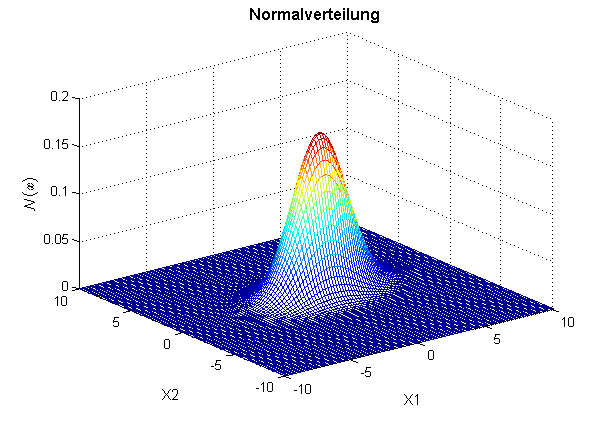
\includegraphics[scale=0.7]{bilder/multivariate_gauss.png}
	\caption{Normalverteilung}
	\label{fig:normalverteilung}
\end{figure}

Im Gegensatz zu fr?heren Webseiten m?ssen wir zum Beispiel nicht mehr zwei verschiedene Webseiten f?r den Internet Explorer und einen anderen Browser programmieren. Es reicht eine Seite, die - richtig angelegt - sowohl auf verschiedenen Browsern im Netz funktioniert, aber ebenso gut f?r den Ausdruck oder die Darstellung auf einem Handy geeignet ist. Wohlgemerkt: Eine Seite f?r alle Formate. Was f?r eine Erleichterung. Standards sparen Zeit bei den Entwicklungskosten und sorgen daf?r, dass sich Webseiten sp?ter leichter pflegen lassen. Nat?rlich nur dann, wenn sich alle an diese Standards halten.